
\documentclass[8pt]{beamer}

\usepackage[english]{babel}
\usepackage[utf8]{inputenc}
\usepackage{pdfpages}
\usepackage{color}
\usepackage{graphicx, import}
\usepackage{amsmath}
\usepackage{amssymb}
\usepackage{amsthm}
\usepackage{tikz}
\usepackage{tabularx}
\usepackage[numbers, square]{natbib}
\usepackage{mathtools}
\usepackage{booktabs}

\usetikzlibrary{positioning, fit, patterns, snakes, chains, arrows, decorations.markings}
%\tikzexternalize[prefix=out/figures/]
\newcolumntype{Y}{>{\centering\arraybackslash}X} % centered equidistant columns

\bibliographystyle{plainnat}
\usetheme{metropolis}
\setbeamertemplate{frame footer}{\insertshortauthor\hfill\insertshortinstitute}
\setbeamercolor{footline}{fg=gray}


\title[]{Weakly Supervised 2D to 3D Lifting of Human Poses}
\author[Nikolas Klug]{Nikolas Klug}
\institute[University of Augsburg]{University of Augsburg}
\date{22 August 2019}


\begin{document}
	{
	\setbeamertemplate{footline}{}
	\begin{frame}
		\titlepage
	\end{frame}
	}
	\addtocounter{framenumber}{-1}

	\begin{frame}
		\begin{figure}
			\vspace{1cm}
			\begin{tikzpicture}
				[
				start chain = A going right,
				txt/.style = {text height=2ex, text depth=0.25ex, font=\sffamily\bfseries\Large,
					on chain},
				every edge/.append style = {draw, -stealth'}
				]
					\node [txt] (weakly) [] {Weakly Supervised};
					{\visible<3->{\draw
					[thick,
					decoration={brace, mirror, raise=0.2cm},
					decorate,
					align=center
					] 
					(weakly.west) -- (weakly.east) node [pos=0.5,anchor=north,yshift=-0.55cm] {using a \\ Generative Adversarial Network \\ -- no ground truth data required};}}
					\node [txt] [right=.2 of weakly] (2Dto3D) [] {2D to 3D Lifting of Human Poses};
					{\visible<1->{\draw 
					[thick,
					decoration={brace, mirror, raise=0.2cm},
					decorate,
					] 
					(2Dto3D.west) -- (2Dto3D.east) node [pos=0.5,anchor=north,yshift=-0.55cm] {};}}
					\visible<1->{
						\node [below left=2cm and -2cm of 2Dto3D] (2Dpose) {\scalebox{-1}[1]{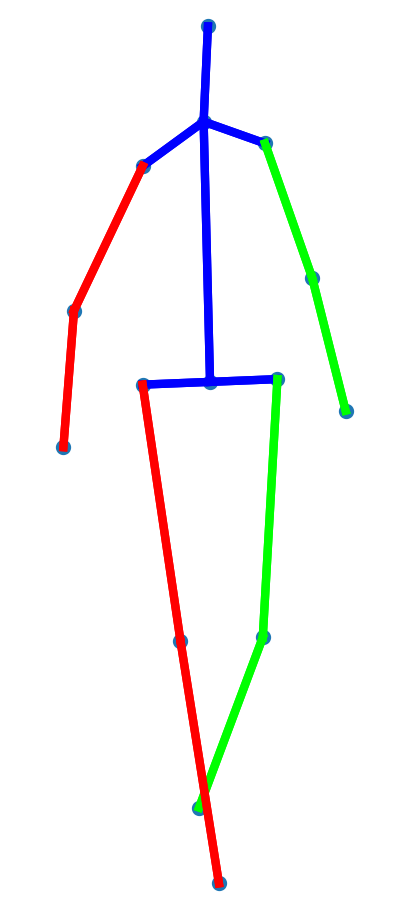
\includegraphics[height=3.2cm]{figures/2D_pose_426411.png}}};
						\node [below right=2cm and -3cm of 2Dto3D] (3Dpose) {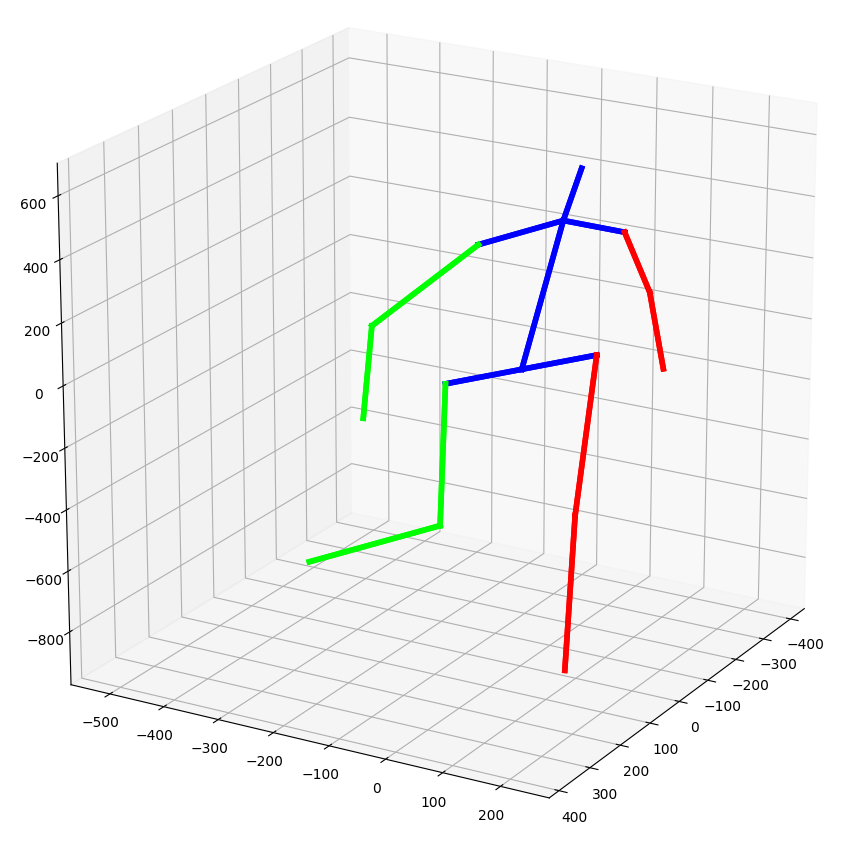
\includegraphics[height=3.2cm]{figures/3D_pose_426411.png}};
						\node [below= 0cm of 2Dpose] (2Dtext) [] {2D pose};
						\node [below= 0cm of 3Dpose] (3Dtext) [] {3D pose};
						\draw [dashed, decoration={markings,mark=at position 1 with
							{\arrow[scale=2,>=stealth]{>}}},postaction={decorate}] (2Dpose.east) -- (3Dpose.west);
						\node[fit=(2Dpose)(3Dpose)(2Dtext)(3Dtext)] (poses) {};
						\draw [decoration={markings,mark=at position 1 with
							{\arrow[scale=2,>=stealth]{>}}},postaction={decorate}] ([yshift=-0.2cm]2Dto3D.south) -- ([yshift=-1.5cm]2Dto3D.south);
					}
			\end{tikzpicture}
		\end{figure}
	\end{frame}

	\begin{frame}{Source}
		\textbf{Can 3D Pose be Learned from 2D Projections Alone?}\linebreak
		\begin{footnotesize}
			Dylan Drover, Rohith MV, Ching-Hang Chen, Amit Agrawal, Ambrish Tyagi, and Cong Phuoc Huynh.\linebreak
			In Computer Vision -- ECCV 2018 Workshops, Pages 78-94, 2019. Springer International Publishing.
		\end{footnotesize}
	\end{frame}

	\begin{frame}{Why?}
		\begin{itemize}
			\item Massive amount of 2D images/videos available
			\item Very good 2D keypoint detectors out there: Stacked Hourglass, OpenPose etc.
			\item Acquiring 3D ground truth data is cumbersome and expensive
		\end{itemize}
	\end{frame}

	\begin{frame}{Underlying heuristic}
		\textbf{If a random 2D projection of a 3D pose looks realistic, the 3D pose is realistic.}
	\end{frame}

	\begin{frame}{How It Works}
		\begin{figure}
			\centering
			\makebox[\textwidth][c]{
				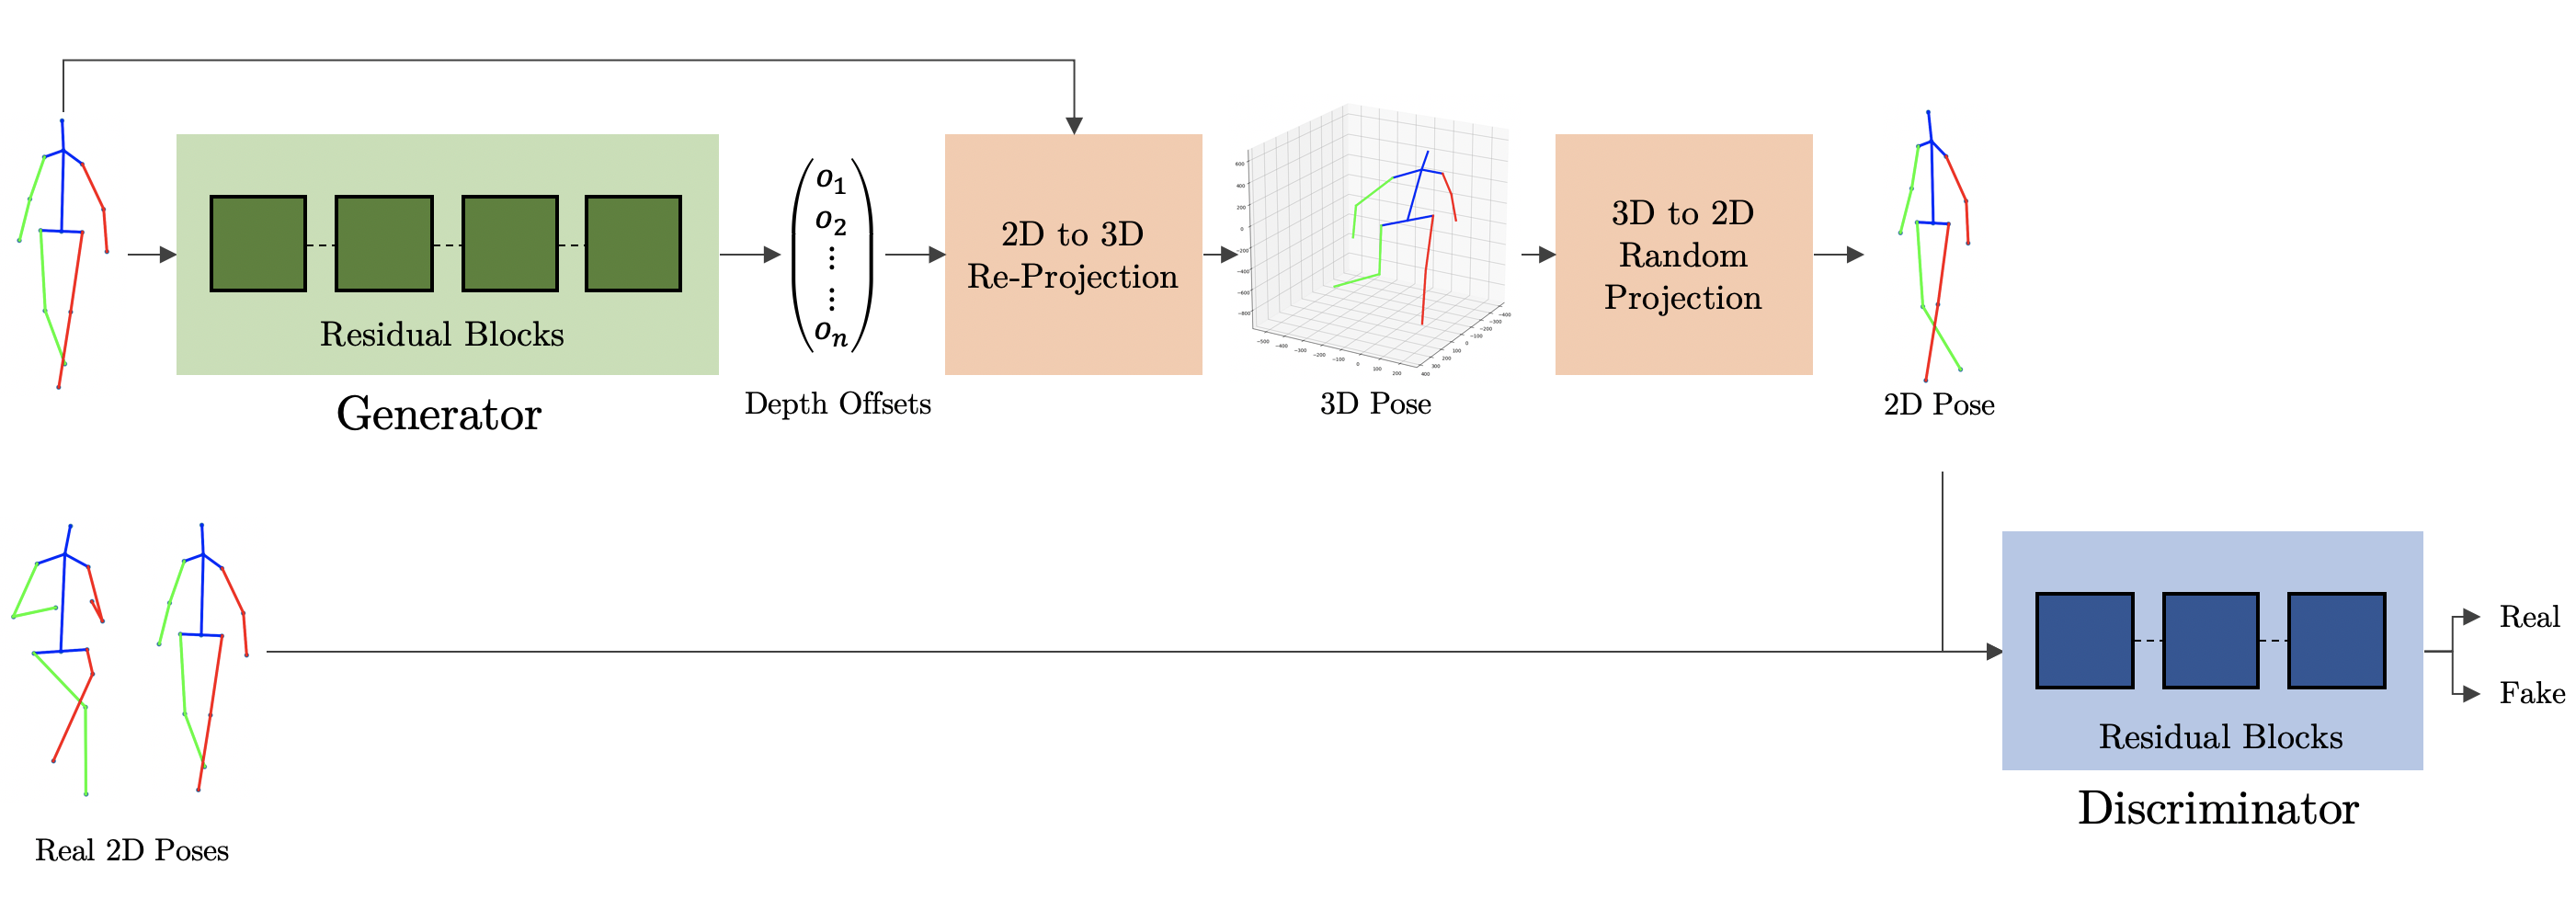
\includegraphics[width=1.1\textwidth]{figures/system.png}
			}                
		\end{figure}
	\end{frame}

	\begin{frame}{Results}
		\begin{table}
			\centering
			\begin{tabularx}{\textwidth}{l *{8}{Y}}
				\toprule
				Method & Direct. & Discuss & Eat & Greet & Phone & Pose & Purchase & Sit \\
				\midrule
				w/o rotation & 48.8 & 51.5 & 41.5 & 57.7 & 49.4 & 54.3 & 48.8 & 50.0 \\
				w/ rotation & 36.3 & 35.5 & 35.6 & 42.6 & 34.8 & 44.1 & 45.2 & 36.3 \\
				\bottomrule
				\toprule
				Method & SitDown & Smoke & TPhoto & Wait & Walk & WDog & WTog. & \textbf{Avg.}\\
				\midrule
				w/o rotation & 64.3 & 51.9 & 64.6 & 57.1 & 54.3 & 57.9 & 53.2 & \textbf{54.8} \\
				w/ rotation  & 51.9 & 41.9 & 50.8 & 43.0 & 38.5 & 49.6 & 40.8 & \textbf{41.0} \\
				\bottomrule
			\end{tabularx}
		\caption{Results for synthetic poses from the Human3.6M dataset with and without rotation to fit the estimated poses to the ground truth data.}
		\end{table}
	\end{frame}
	
	\begin{frame}{My Contribution}
		\begin{itemize}
			\item Introduction of \emph{Limb Loss}
			\item Analysis of the effects of pose normalization 
		\end{itemize}
	\end{frame}
	
	
\end{document}